\section{Concept}
To be able to meet the requirements of our interactive floorplan, the events from the gate need to be logged and displayed in real-time. For this to work, there a multiple component involved. A general overview about the architecture can be seen in figure 3.1.

\begin{figure}[!hb]
	\centering
	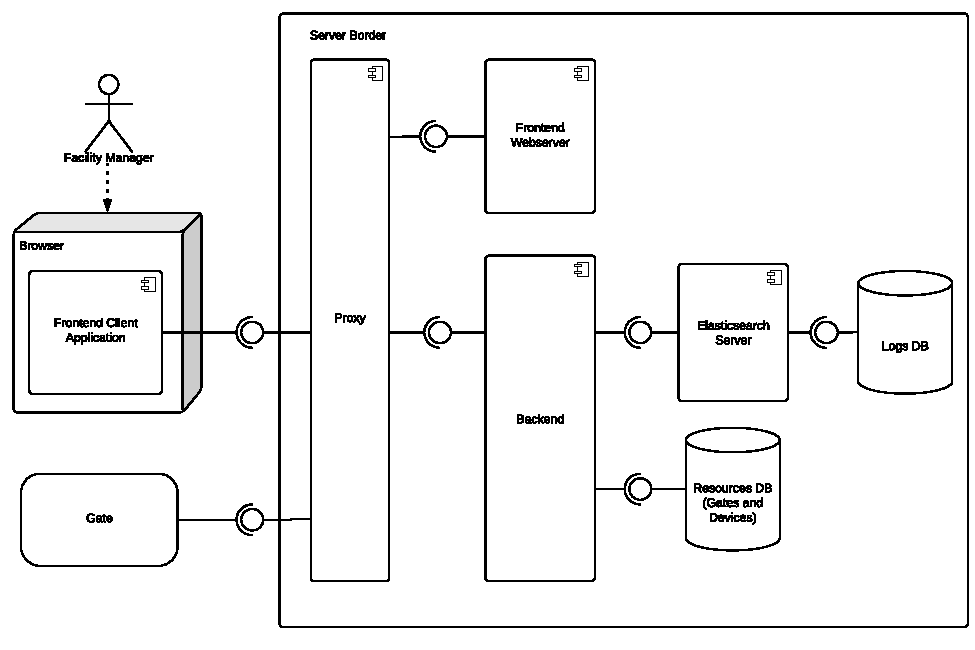
\includegraphics[width=0.9\linewidth]{images/Komponentendiagramm}
	\caption{Component diagram}
	\label{fig:Komponentendiagramm}
\end{figure}

\subsection{Gates}
\label{Gates}

The gates take care of capturing different informations once a person tries to enter a gate. They retrieve information about the device that communicates with them, if they granted or denied the access and if the person tried to enter or exit through the gate.

The gate then is responsible of sending this information to our system via an API.

If an alarm occured at a gate they need to provide specific information to our backend.

\subsection{Backend}
\label{Backend}

The backend offers interfaces for the gates and also the frontend. For the gates it provides an interface which allows the gates to send events to, which then will be persisted as logs.
For the frontend it provides routes for retrieving logs and also other results based on these.

It emits a notification together with the event data once a gate event occured for a real time frontend application.


\subsection{Frontend}
\label{Frontend}

The frontend presents the interactive floorplan to the facility management with clickable markers for each gate.
It features the adding an deleting of marker and the possibility to link them to a gate.
A click on a specific marker shows useful informations about the gate, such as the minimal entry and minimal exit trust level required for this gate.

For the possibility of displaying data in real-time, it listens for the gate event notification sent from the backend. When an event occurs the frontend reads in the gate event informationen. With this it finds out who accessed at which gate and presents that information to the facility management. It then asks for the backend for an updated number of people behind that specific gate. It than calculates the heat in that specific an rerenders the color of that room accordingly.

\subsection{Elasticsearch Server}
\label{Elasticsearch Server}

angeschlossen an DB, bietet interface fuer anlegen von event logs und auslesen von event logs + suche





